%%==================================================
%% ch2.tex for BIT Master Thesis
%% modified by yang yating
%% version: 0.5
%% last update: April 25th, 2017
%%==================================================

\chapter{模板使用}
\label{chap:textStructure}

本章的目的是介绍\LaTeX{}的文本控制流程,介绍学位论文中各章节分布以及模板内部组成,以及章节内的交叉引用问题,用户可以根据自身对\LaTeX{}的熟悉程度适当地略过阅读。在了解了本章的内容后,用户即可通过文本内容的粘贴和复制,快速实现生成一个格式满足基本需求的学位论文。

以硕士模板BIT-thesis-template-grd为例,文件布局如图 \ref{layout-master} 所示。 

\begin{lstlisting}[basicstyle=\small\ttfamily,caption={BIT-thesis-template-grd 模板文件布局},label=layout-master,numbers=none]
  ├── demo.tex              主控文件
  ├── demo.pdf              生成的论文pdfBIT-thesis-template-grd
  ├── BIT-thesis-grd.cls    格式控制文件
  ├── GBT7714-2005NLang.bst 参考文献格式控制文件
  ├── chapters              章节文件夹
  │   ├── abstract.tex       摘要
  │   ├── chapter01.tex      第一章
  │   ├── conclusion.tex     总结
  │   ├── app1.tex           附录A
  │   ├── pub.tex            攻读学位期间发表论文与研究成果清单
  │   └── thanks.tex         致谢
  ├── figures               图片文件夹
  │   └── figure1.png   
  ├── reference             参考文献文件夹
  │   └── chap1.bib
  ├── BIT-thesis-run.cmd    运行脚步cmd
  └── BIT-thesis-run.sh     运行脚本sh
  
      
\end{lstlisting}

\section{认识模板组成}

\subsection{格式控制文件}
\label{sec:format}

格式控制文件控制着论文的表现形式,包括以下两个文件:BIT-thesis-grd.cls 和 GBT7714-2005NLang.bst。
其中,``.cls''控制论文主体格式,``.bst''控制参考文献条目的格式,

一般用户可以``忽略''格式控制文件的存在。因为该文件已经按照《北京理工大学博士、硕士学位
论文撰写规范》进行了修改。有其他格式修改的需要,参见第\ref{sec:thesisformat}章。


\subsection{主控文件~demo.tex}
\label{sec:demotex}

主控文件~demo.tex~的作用就是将分散在多个文件中的内容``整合''成一篇完整的论文。
使用这个模板撰写学位论文时,学位论文内容和素材会被``拆散''到各个文件中:
譬如各章正文、各个附录、各章参考文献等等。
在~demo.tex~中通过``include''命令将论文的各个部分包含进来,从而形成一篇结构完成的论文。
封面页中的论文标题、作者等中英文信息,也是在~demo.tex~中填写。也可以在demo.tex中按照自己的需要引入一些的宏包
\footnote{一般只有当你需要在文档中使用那个宏包时,才需要在导言区中用~usepackage~引入该宏包。如若不然,通过usepackage引入一大堆不被用到的宏包,必然是一场灾难。由于一开始没有一致的设计目标,\LaTeX~ 的各宏包几乎都是独立发展起来的,因重定义命令导致的宏包冲突屡见不鲜。}。

大致而言,在主控文件~demo.tex~中,只需要留意文章有哪些章节以及各章参考文
献内容,不需要具体关注每一章里面的具体内容。需要注意,处理文档时所有的操作命令
{}\cndash{}xelatex, bibtex等,都是作用在~demo.tex~上,而\emph{不是}后面这
些``分散''的文件,请参考\ref{sec:process}小节。

若使用\textbf{硕士论文模板},请在~demo.tex~中~\verb|\documentclass|~命令采用~master~选项;若使用\textbf{博士论文模板},请使用~doctor~选项。同理,单页打印使用~oneside~选项,双面打印使用~twoside~选项。

文章各部分安排如下:
\begin{itemize}
\item ~\verb|\maketitle|~ : 中文封面
\item ~\verb|\makeInfo|~ : 中文信息
\item ~\verb|\makeEnglishInfo|~ : 英文信息
\item ~\verb|\makeVerticalTitle|~ : 打印竖排论文题目
\item ~\verb|\makeDeclareOriginal|~ : 论文原创性声明和使用授权
\item ~\verb|%
%
%

\begin{abstract}
  本文……。({\color{blue}{摘要是一篇具有独立性和完整性的短文,应概括而扼要地反映出本论文的主要内容。包括研究目的、研究方法、研究结果和结论等,特别要突出研究结果和结论。中文摘要力求语言精炼准确,硕士学位论文摘要建议500~800字,博士学位论文建议1000~1200字。摘要中不可出现参考文献、图、表、化学结构式、非公知公用的符号和术语。英文摘要与中文摘要的内容应一致。}})

  \keywords{形状记忆;聚氨酯;织物;合成;应用 ({\color{blue}{一般选3~8个单词或专业术语,且中英文关键词必须对应。})}}
\end{abstract}

\begin{abstractEN}
  In order to exploit ……

  \keywordsEN{shape memory properties; polyurethane;textile;synthesis;application}
\end{abstractEN}
|~ :摘要
\item ~\verb|\tableofcontents|~ :加入目录
\item ~\verb|\listoftables|~ :加入表格索引
\item ~\verb|\listoffigures|~ : 加入插图索引
\item ~\verb|%
%
%

\chapter{绪论}
\label{chap:intro}

\section{本论文研究的目的和意义}

近年来,随着人们生活水平的不断提高,人们越来越注重周围环境对身体健康的影响。作为服装是人们时时刻刻最贴近的环境,尤其是内衣,对人体健康有很大的影响。由于合时刻刻最贴近的环境,尤其是内衣,对人体健康有很大的影响。由于合成纤维的衣着舒适性、手感性,天然纤维的发展又成为人们关注的一大热点。

……

\section{国内外研究现状及发展趋势}

\subsection{形状记忆聚氨酯的形状记忆机理}

形状记忆聚合物(SMP)是继形状记忆合金后在80年代发展起来的一种新型形状记忆材料。形状记忆高分子材料在常温范围内具有塑料的性质,即刚性、形状稳定恢复性;同时在一定温度下(所谓记忆温度下)具有橡胶的特性,主要表现为材料的可变形性和形变恢复性。即“记忆初始态-固定变形-恢复起始态”的循环。

固定相只有物理交联结构的聚氨酯称为热塑性SMPU,而有化学交联结构称为热固性SMPU。热塑性和热固性形状记忆聚氨酯的形状记忆原理示意图如图\ref{fig:diagram}所示。

\begin{figure}
  \centering
  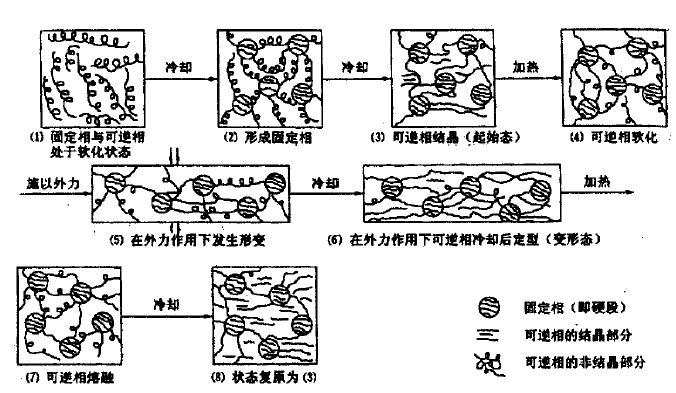
\includegraphics[width=0.75\textwidth]{assets/figure1.png}
  \caption{热塑性形状记忆聚氨酯的形状记忆机理示意图}
  \label{fig:diagram}
\end{figure}

\subsection{形状记忆聚氨酯的研究进展}

首例SMPU是日本Mitsubishi公司开发成功的……。

\subsection{水系聚氨酯及聚氨酯整理剂}

水系聚氨酯的形态对其流动性,成膜性及加工织物的性能有重要影响,一般分为三种类型\cite{Jiang2005Size} ,如表\ref{tab:category}所示。

\begin{table}
  \centering
  \caption{水系聚氨酯分类}
  \label{tab:category}
  \begin{tabular*}{0.9\textwidth}{@{\extracolsep{\fill}}cccc}
    \toprule
      类别			&水溶型		&胶体分散型		&乳液型 \\
    \midrule
      状态			&溶解$\sim$胶束	&分散		&白浊 \\
      外观			&水溶型		&胶体分散型		&乳液型 \\
      粒径$/\mu m$	&$<0.001$		&$0.001-0.1$		&$>0.1$ \\
      重均分子量	&$1000\sim 10000$	&数千$\sim 20万$ &$>5000$ \\
    \bottomrule
  \end{tabular*}
\end{table}

由于它们对纤维织物的浸透性和亲和性不同,因此在纺织品染整加工中的用途也有差别,其中以水溶型和乳液型产品较为常用。另外,水系聚氨酯又有反应性和非反应性之分。虽然它们的共同特点是分子结构中不含异氰酸酯基,但前者是用封闭剂将异氰酸酯基暂时封闭,在纺织品整理时复出。相互交联反应形成三维网状结构而固着在织物表面。

……
|~ : 各章正文内容
\item ~\verb|%%==================================================
%% modified based on BIT-Thesis-template v1.5
%% author: Zheng Shuai <i AT iamzs.win>
%%==================================================

\begin{conclusion}

  本文采用……。{\color{blue}(结论作为学位论文正文的最后部分单独排写,但不加章号。结论是对整个论文主要结果的总结。在结论中应明确指出本研究的创新点,对其应用前景和社会、经济价值等加以预测和评价,并指出今后进一步在本研究方向进行研究工作的展望与设想。结论部分的撰写应简明扼要,突出创新性。)}

\end{conclusion}
|~ : 结论
\item ~\verb|\bibliography{reference/chap1}|~ :参考文献
\item ~\verb|%%==================================================
%% app1.tex for BIT Master Thesis
%% modified by yang yating
%% version: 0.1
%% last update: Dec 25th, 2016
%%==================================================


\chapter{***}

附录相关内容…
 |~ : 附录
\item ~\verb|%%==================================================
%% pub.tex for BIT Master Thesis
%% modified by yang yating
%% version: 0.1
%% last update: Dec 25th, 2016
%%==================================================

\begin{publications}{99}

    \item\textsc{高凌}. {交联型与线形水性聚氨酯的形状记忆性能比较}[J].
      化工进展, 2006, 532-535.(核心期刊)
    
\end{publications}
|~ : 攻读学位期间发表论文与研究成果清单
\item ~\verb|%%==================================================
%% thanks.tex  for BIT Master Thesis
%% modified by yang yating
%% version: 1.0
%% last update: Sep 8th, 2017
%%==================================================


\begin{thanks}


感谢计算机学院2016级研究生杨雅婷对本模板的撰写与更新做了大量工作。特别感谢宇航学院2015级硕士研究生汪卫对本模板更新与维护所做的突出贡献。同时,由衷感谢在Github对该项目上提出大量珍贵修改意见的老师和同学们。

本项目得到研究生院学位与学部办公室和学生事务中心的资助支持。

\end{thanks}
|~ : 致谢
\item ~\verb|%%==================================================
%% resume.tex  for BIT Master Thesis
%% modified by yang yating
%% version: 0.2
%% last update: Feb 16th, 2017
%%==================================================


\begin{resume}

\begin{resumesection}{基本情况}
xxx,男,上海人,1985 年~12 月出生,未婚,
上海交通大学物理系在读博士研究生。
\end{resumesection}

\begin{resumeli}{教育状况}
XXXX 年~9 月至~XXXX 年~7 月,上海交通大学, 本科,专业:XXXX

XXXX 年~9 月至~XXXX 年~7 月,上海交通大学, 硕士研究生,专业:XXXX

XXXX 年~9 月至~XXXX 年~7 月,上海交通大学,
博士研究生(提前攻读博士),专业:XXXX
\end{resumeli}

\begin{resumeli}{工作经历}
无。
\end{resumeli}

\begin{resumeli}{研究兴趣}
XXXXXXX。
\end{resumeli}

\begin{resumeli}{联系方式}
通讯地址:上海市闵行区东川路800号,上海交通大学物理系

邮编:200240

E-mail: abcde@sjtu.edu.cn
\end{resumeli}

\end{resume}
|~ : 作者简介(博士论文需要)
\end{itemize}


\subsection{论文主体文件夹chapters}
\label{sec:thesisbody}

这一部分是论文的主体,是以``章''为单位划分的。

正文前部分(frontmatter):中英文摘要(abstract.tex)。其他部分,诸如中英文信息封
面、授权信息等,都是根据~demo.tex~所填的信息自动生成好了,不需要单独编写文件。

正文部分(mainmatter):是各章内容,在chapter文件夹中。

正文后的部分(backmatter):附录(app\emph{xx}.tex);致谢(thanks.tex);攻读
学位论文期间发表的学术论文目录(pub.tex);作者简介(resume.tex)。参考文献列
表是自动生成的,也不需要作为一个单独的文件。另外,学校的硕士研究生学位论文模
板没有要求加入作者简介,但\textbf{博士的学位论文要求加入作者简介}。


\subsection{图片文件夹~figures}
\label{sec:figuresdir}

figures~文件夹放置了需要插入文档中的图片文件(PNG/JPG/PDF/EPS)。如果图片较多,建议按章再
划分子目录存储图片。

\subsection{参考文献数据库文件夹~reference}
\label{sec:bibdir}

reference~文件夹放置的是各章``可能''会被引用的参考文献文件。参考文献的元
数据,例如作者、文献名称、年限、出版地等,会以一定的格式记录在纯文本文
件.bib中。最终的参考文献列表是BibTeX处理.bib后得到的,名为~demo.bbl。将参
考文献按章划分的一个好处是,可以在各章后生成独立的参考文献,不过,现在看
来没有这个必要。关于参考文献的管理,可以进一步参考第\ref{chap:example}章
中的例子。


\section{进行论文写作}
\label{sec:format}

本节介绍使用论文模板,修改论文信息、摘要、关键字,以及编辑章节等。

\subsection{封面和标题}
在主控文件demo.tex中填写论文的相应信息。

中文封面信息:
\begin{itemize}
\item 中图分类号(\verb|\classification{TQ028.1}|)
\item UDC分类号(\verb|\UDC{540}|)
\item 论文标题(\verb|\title{论文标题}|)
\item 作者姓名(\verb|\author{姓名}|)
\item 学院名称(\verb|\institute{学院名称}|)
\item 指导教师(\verb|\advisor{教授姓名}|)
\item 答辩委员会主席(\verb|\chairman{教授姓名}|)
\item 申请学位(\verb|\degree{学位名称}|)
\item 学科专业(\verb|\major{专业名称}|)
\item 学位授予单位(\verb|\school{北京理工大学}|)
\item 论文答辩日期(\verb|\defenddate{答辩日期}|)
\end{itemize}


英语封面信息:
\begin{itemize}
\item English Title(\verb|\englishtitle{论文标题}|)
\item Candidate Name(\verb|\englishauthor{姓名}|)
\item School or Department(\verb|\englishinstitute{学院名称}|)
\item Faculty Mentor(\verb|\englishadvisor{教授姓名}|)
\item Chair,Thesis Committee(\verb|\englishchairman{教授姓名}|)
\item Degree Applied(\verb|\englishdegree{学位名称}|)
\item Major(\verb|\englishmajor{专业名称}|)
\item Degree by(\verb|\englishschool{Beijing Insititute of Technology}|)
\item The Data of Defence(\verb|\englishdate{答辩日期}|)
\end{itemize}

\subsection{摘要和关键字}
摘要内容,放置于chapters文件夹下的abstract.tex中,

中文摘要于\verb|abstract|环境编写;\verb|\keywords|为中文关键字。英文摘要于\verb|englishabstract|环境编写;\verb|\englishkeywords|为中文关键字。

\begin{lstlisting}[language={[LaTeX]TeX}, caption={ 中英文摘要 }]
\begin{abstract}
	本文 ...
\keywords { 形状记忆;聚氨酯 }
\end{abstract}

\begin{englishabstract}
   In order to exploit ...
\englishkeywords{shape memory properties; polyurethane}
\end{englishabstract}
\end{lstlisting}


\subsection{正文章节}
章节的设置分别通过关键字完成,按照章节的级别依此如表~\ref{tab:setSection}所示,关于文档中具体章节的关键词设置可以参看原宏包中tex文件夹下的实例文件。

\begin{table}[htb]
 \centering
  \caption{章节设置关键字}     % title of Table
  \label{tab:setSection}    % label of Table
  \begin{tabular}{cl}
    \hline
    章节级别        & 关键字     \\
    \hline
     章        & \verb|\chapter| \\
     节        & \verb|\section | \\
    子节      & \verb|\subsection |\\
    表格名称       & \verb|\caption{标题名称}| \\
    引用标签       & \verb|\label{引用名称}| \\
    \hline
  \end{tabular}
\end{table}

\subsection{其他部分}


全文总结、攻读学位期间发表论文与研究成果清单、致谢的内容,均位于chapters文件夹下,分别为conclusion.tex,pub.tex,thanks.tex。

\section{交叉引用}
\subsection{公式、图表和插图引用}
\label{sec:refofFigAndTab}
交叉引用的前提是需要在定义章节、公式和图表的时候都对其进行命名标签(即\textbackslash label\{sec:labelName\}命令),在实际使用过程中通过标签进行引用。根据引用的特点可以将应用分成表~\ref{tab:citeType}中所示三类。

\begin{table}[htb]
 \centering
  \caption{交叉引用类型}       % title of Table
  \label{tab:citeType}    % label of Table
  \begin{tabular}{cl}
    \hline
    引用类型     & 关键字     \\
    \hline
    标签设置        & \textbackslash label\{marker\}  \\
    引用代号        & \textbackslash ref\{marker\}    \\
    引用页码        & \textbackslash pageref\{marker\} \\
    引用文献        & \textbackslash cite\{regLabel\} \\
    \hline
  \end{tabular}
\end{table}

其中,表格和图片的摆放位置由 \textbackslash begin\{table\}或\textbackslash begin\{figure\}后面的中括号设置,例如[htb]表示可以将图表放在当前位置(here)、页面顶端(top)或者页面底端(bottom)。

{\bf{实例1:}}这里是对表格《交叉引用类型》的引用——表~\ref{tab:citeType}位于第~\pageref{tab:citeType}页,其标签为\textbackslash label\{tab:citeType\}。


\subsection{文献引用}
\label{sec:citeRefs}

BIT-Thesis论文模板使用BibTeX处理参考文献。

参考文献的具体内容就是reference文件夹下的chap\textit{xx}.bib,参考文献的元数据(名称、作者、出处等)以一定的格式保存在这些纯文本文件中。
.bib文件也可以理解为参考文献的``数据库'',正文中所有引用的参考文件条目都会从这些文件中``析出''。

正文中引用参考文献时,用\verb+\upcite{...}+可以产生“上标引用的参考文献”,
如\upcite{chen2007act},\upcite{Meta_CN,chen2007act,DPMG}。

具体使用方法参见第\ref{sec:reference}节。
